\documentclass{article}
\usepackage[utf8]{inputenc}
\usepackage[T1]{fontenc}
\usepackage[italian]{babel}
\usepackage{geometry}
\usepackage{graphicx}
\geometry{a4paper, margin=1in}

\title{Capitolo 10 - Sicurezza del Sistema Operativo}
\author{}
\date{}

\begin{document}

\maketitle

\section*{Il Ruolo del Sistema Operativo nella Sicurezza}

Il Sistema Operativo (OS) rappresenta la prima linea di difesa di un'infrastruttura informatica. Il suo compito primario è proteggere gli utenti l'uno dall'altro, garantendo che aree critiche di memoria o di archiviazione non vengano sovrascritte da processi non autorizzati. Inoltre, l'OS si occupa di eseguire l'identificazione e l'autenticazione delle persone e delle operazioni remote, assicurando un'equa condivisione delle risorse hardware critiche. Proprio per questa sua posizione centrale, il sistema operativo è il bersaglio principale degli attacchi: compromettere con successo l'OS significa ottenere il controllo completo sulla macchina e su tutti i suoi componenti.

Tra le funzioni principali del sistema operativo che coinvolgono la sicurezza informatica troviamo:

\begin{itemize}
    \item \textbf{Condivisione forzata (Enforced sharing):} le risorse dovrebbero essere rese disponibili agli utenti in modo appropriato. Questo comporta la necessità di garantire integrità e coerenza.
    \item \textbf{Comunicazione interprocesso e sincronizzazione:} l'OS funge da ponte tra i processi, rispondendo alle richieste dei processi per la comunicazione asincrona con altri processi o per la sincronizzazione. La comunicazione interprocesso è mediata da tabelle di controllo degli accessi.
    \item \textbf{Protezione dei dati critici del sistema operativo:} l'OS deve mantenere i dati attraverso i quali può far rispettare la sicurezza. Se questi dati non sono protetti da accessi non autorizzati (lettura, modifica e cancellazione), il sistema operativo non può imporre il rispetto delle regole.
    \item \textbf{Servizio equo garantito (Guaranteed fair service):} necessità di evitare la starvation (morte per inedia) di utenti/processi (per garantire la disponibilità). I clock hardware si combinano con le discipline di scheduling per fornire equità. Le funzionalità hardware e le tabelle di dati si combinano per fornire controllo.
    \item \textbf{Interfaccia verso l'hardware, File e dispositivi di I/O:} mediare e controllare l'accesso ai dispositivi hardware, ai dispositivi di I/O e al File system (controllo degli accessi).
    \item \textbf{Autenticazione dell'utente:} Il sistema operativo deve identificare ciascun utente che richiede l'accesso e deve accertarsi che l'utente sia effettivamente chi dichiara di essere.
    \item \textbf{Protezione della memoria:} per garantire che lo spazio utente/sistema non venga violato (CIA - Confidenzialità, Integrità, Disponibilità).
\end{itemize}

\vspace{0.8cm}

\section*{Architettura e Protezione dei Livelli}

\vspace{0.3cm}
\noindent \begin{minipage}{0.48\textwidth}
    La progettazione del sistema operativo deve mirare a proteggere una vasta gamma di oggetti, tra cui la memoria, i dispositivi I/O condivisibili (come i dischi) o riutilizzabili serialmente (come le stampanti), i programmi, le reti e i dati condivisi. Per fare ciò, i sistemi operativi moderni adottano una visione stratificata (layered view). Al centro risiede il \textit{Security Kernel}, che impone le regole di sicurezza, circondato dall'\textit{Operating System Kernel}, che alloca le risorse primitive come il tempo o l'accesso all'hardware. Attorno a questi si sviluppano le funzioni di utilità e, infine, i processi utente.
\end{minipage}
\hfill
\begin{minipage}{0.48\textwidth}
    \centering
    \includegraphics[width=\textwidth]{Screenshot 2026-05-04 alle 13.07.55.png}
\end{minipage}

\vspace{0.8cm}

\noindent \begin{minipage}{0.48\textwidth}
    Questo approccio si traduce in una "visione a cipolla" (onion-ring view) dove il codice più fidato (Most Trusted Code) si trova al centro (ad esempio, l'aggiornamento dei dati di autenticazione), mentre man mano che ci si sposta verso l'esterno si trova codice sempre meno fidato, fino ad arrivare all'interfaccia utente.
\end{minipage}
\hfill
\begin{minipage}{0.48\textwidth}
    \centering
    \includegraphics[width=\textwidth]{Screenshot 2026-05-04 alle 13.08.04.png}
\end{minipage}

\vspace{0.8cm}

La natura multi-componente dei sistemi operativi tuttavia rappresenta anche una potenziale breccia per la sicurezza. I moduli dell'OS provengono da fonti diverse, non tutte affidabili, e devono integrarsi con successo. Pertanto, l'OS deve proteggere se stesso \textbf{sia da programmi utente errati o malevoli, sia dai danni causati da moduli aggiuntivi o driver di cui non si conosce appieno il livello di affidabilità}. Nei primi sistemi degli anni '70 e '80, sviluppati per hardware specifici (come la famiglia VAX o i sistemi BiiN), la protezione era fortemente applicata e supportata a livello hardware, con molteplici livelli di separazione distinti. Nei sistemi operativi odierni, che girano su hardware generico, questo tipo di supporto nativo non può essere sfruttato allo stesso modo.

\vspace{0.8cm}

\section*{Strumenti per le Funzionalità di Sicurezza e Utilità}

Per implementare le funzioni di controllo, l'OS utilizza strumenti come le ACL (Access Control List), liste di privilegi e capabilities. Il sistema operativo gestisce le tabelle sottostanti e i meccanismi che verificano la validità delle richieste. Un'altra funzione vitale è il logging degli eventi (Audit logs), che permette di ricostruire cosa è accaduto durante un incidente e aiuta a prevenire futuri attacchi.

Per quanto riguarda l'isolamento e la gestione delle risorse, esistono diversi concetti applicativi:

\subsection*{Virtualizzazione}

Permette all'OS di presentare a ciascun utente o classe di utenti solo le risorse che dovrebbero vedere, creando l'astrazione della Macchina Virtuale (VM). Un \textit{hypervisor} (o Virtual Machine Monitor) controlla e filtra tutte le richieste provenienti da una VM, eseguendo in modo controllato le istruzioni privilegiate e l'allocazione della memoria.

\subsection*{Sandbox}

È un ambiente controllato in cui un processo ha un impatto limitato sulle risorse esterne. Ad esempio, nel sistema Java originale, il codice fidato ha accesso all'ambiente, mentre il codice non fidato (come un'applet scaricata da internet) viene eseguito nella sandbox. L'ambiente di runtime Java funge da macchina virtuale che vincola le applet in uno spazio sicuro, utilizzando un compilatore e un \textit{bytecode verifier} per garantire la corretta sintassi dei comandi, mentre la Java Virtual Machine agisce da reference monitor per tutte le richieste di accesso.

\subsection*{Honeypot}

Solitamente impiegato nelle reti, mostra un set limitato e sicuro di risorse a un potenziale attaccante. Permette agli analisti di sicurezza di monitorare le attività in tempo reale per scoprire gli obiettivi, le tecniche e gli strumenti dell'attaccante. Lo stesso approccio può essere usato nell'OS eseguendo una VM honeypot per ingaggiare gli avversari e raccogliere informazioni difensive.

\vspace{0.8cm}

\section*{Separazione e Condivisione delle Risorse}

Un pilastro della sicurezza del sistema operativo è il delicato equilibrio tra separazione e condivisione. La separazione può avvenire attraverso diverse dimensioni: può essere \textit{fisica} (processi diversi usano oggetti fisici diversi, come stampanti separate per livelli di sicurezza differenti), \textit{temporale} (processi con requisiti diversi vengono eseguiti in momenti diversi), \textit{logica} (gli utenti operano con l'illusione di essere soli, grazie a un OS che vincola strettamente i domini di accesso) o \textit{crittografica} (i dati vengono resi incomprensibili ai processi esterni).

Tuttavia, la separazione è solo metà della medaglia. È necessario proteggere gli oggetti di un utente, ma anche permetterne la condivisione quando richiesto. Il sistema operativo offre protezione su vari livelli: può decidere di non proteggere affatto (ad esempio se si usa la separazione temporale), di isolare completamente i processi nascondendoli l'uno all'altro, oppure di adottare una politica del tipo "condividi tutto o nulla", dove un oggetto è pubblico per tutti o privato solo per il proprietario. Approcci più granulari permettono di condividere limitando l'accesso tramite regole di \textit{access control}, oppure limitando direttamente l'uso che si può fare di un oggetto dopo avervi effettuato l'accesso (ad esempio, permettendo la visualizzazione di un documento ma bloccandone la stampa).

\vspace{0.8cm}

\section*{Protezione Hardware della Memoria}

Per mantenere isolati i processi, l'hardware offre diversi meccanismi di protezione della memoria:

\vspace{0.3cm}
\noindent \begin{minipage}{0.48\textwidth}
    \begin{itemize}
        \item \textbf{Fence (Recinto statico):} Si tratta di una limitazione hardware fissa degli indirizzi. La memoria è divisa in due blocchi: gli indirizzi da 0 a n sono riservati al sistema operativo, mentre da n+1 in poi risiede lo spazio dei programmi utente.
    \end{itemize}
\end{minipage}
\hfill
\begin{minipage}{0.48\textwidth}
    \centering
    \includegraphics[width=\textwidth]{Screenshot 2026-05-04 alle 13.08.11.png}
\end{minipage}

\vspace{0.5cm}

\noindent \begin{minipage}{0.48\textwidth}
    \begin{itemize}
        \item \textbf{Fence Register (Recinto dinamico):} Utilizza un registro dei limiti di indirizzo che può variare (ad esempio da n+1 a p+1). Questo permette una maggiore flessibilità dinamica per separare l'OS dai programmi utente.
    \end{itemize}
\end{minipage}
\hfill
\begin{minipage}{0.48\textwidth}
    \centering
    \includegraphics[width=\textwidth]{Screenshot 2026-05-04 alle 13.08.19.png}
\end{minipage}

\vspace{0.5cm}

\noindent \begin{minipage}{0.48\textwidth}
    \begin{itemize}
        \item \textbf{Registri Base/Bound:} Questo sistema utilizza due registri. Il \textit{Base Register} indica l'indirizzo di partenza dello spazio consentito, mentre il \textit{Bounds Register} ne indica il limite finale. Questo approccio permette di gestire e proteggere dinamicamente spazi multipli per più utenti contemporaneamente (Utente A, B, C) e può essere ulteriormente raffinato separando il registro base/bound per il Codice (Programma) da quello per i Dati, isolando così lo spazio di esecuzione da quello di archiviazione dati per ogni singolo utente.
    \end{itemize}
\end{minipage}
\hfill
\begin{minipage}{0.48\textwidth}
    \centering
    \includegraphics[width=\textwidth]{Screenshot 2026-05-04 alle 13.08.29.png}
\end{minipage}

\vspace{0.3cm}
\begin{itemize}
    \item \textbf{Tagged Architecture:} Consiste nel controllare ogni singola locazione (parola) di memoria associandovi un "Tag" che ne definisce i diritti di accesso (ad esempio R per Solo Lettura, X per Solo Esecuzione, RW per Lettura/Scrittura).
\end{itemize}

\vspace{0.8cm}

\section*{Memoria Virtuale: Segmentazione e Paginazione}

Per gestire la memoria in modo più flessibile e sicuro, i sistemi operativi utilizzano la memoria virtuale tramite segmentazione e paginazione.

La \textbf{Segmentazione} permette di dividere logicamente un programma in più parti (segmenti come MAIN, SUB, DATA\_SEG) che hanno diritti di accesso differenti. Viene implementata tramite una tabella di traduzione dei segmenti che converte gli indirizzi logici in indirizzi fisici nascondendoli al processo. Nascondere gli indirizzi offre grandi vantaggi: l'OS può spostare i segmenti ovunque, anche in memoria ausiliaria durante l'esecuzione, e poiché ogni riferimento passa attraverso l'OS, c'è la costante opportunità di controllare i permessi di accesso. La segmentazione garantisce che ogni riferimento sia verificato all'interno dei confini del segmento, impedisce la generazione di indirizzi non permessi e permette la condivisione sicura di specifici dati tra utenti. L'unica complessità risiede nel fatto che la dimensione variabile dei segmenti richiede controlli continui per evitare che un indirizzo sfori la lunghezza del segmento stesso.

\begin{center}
    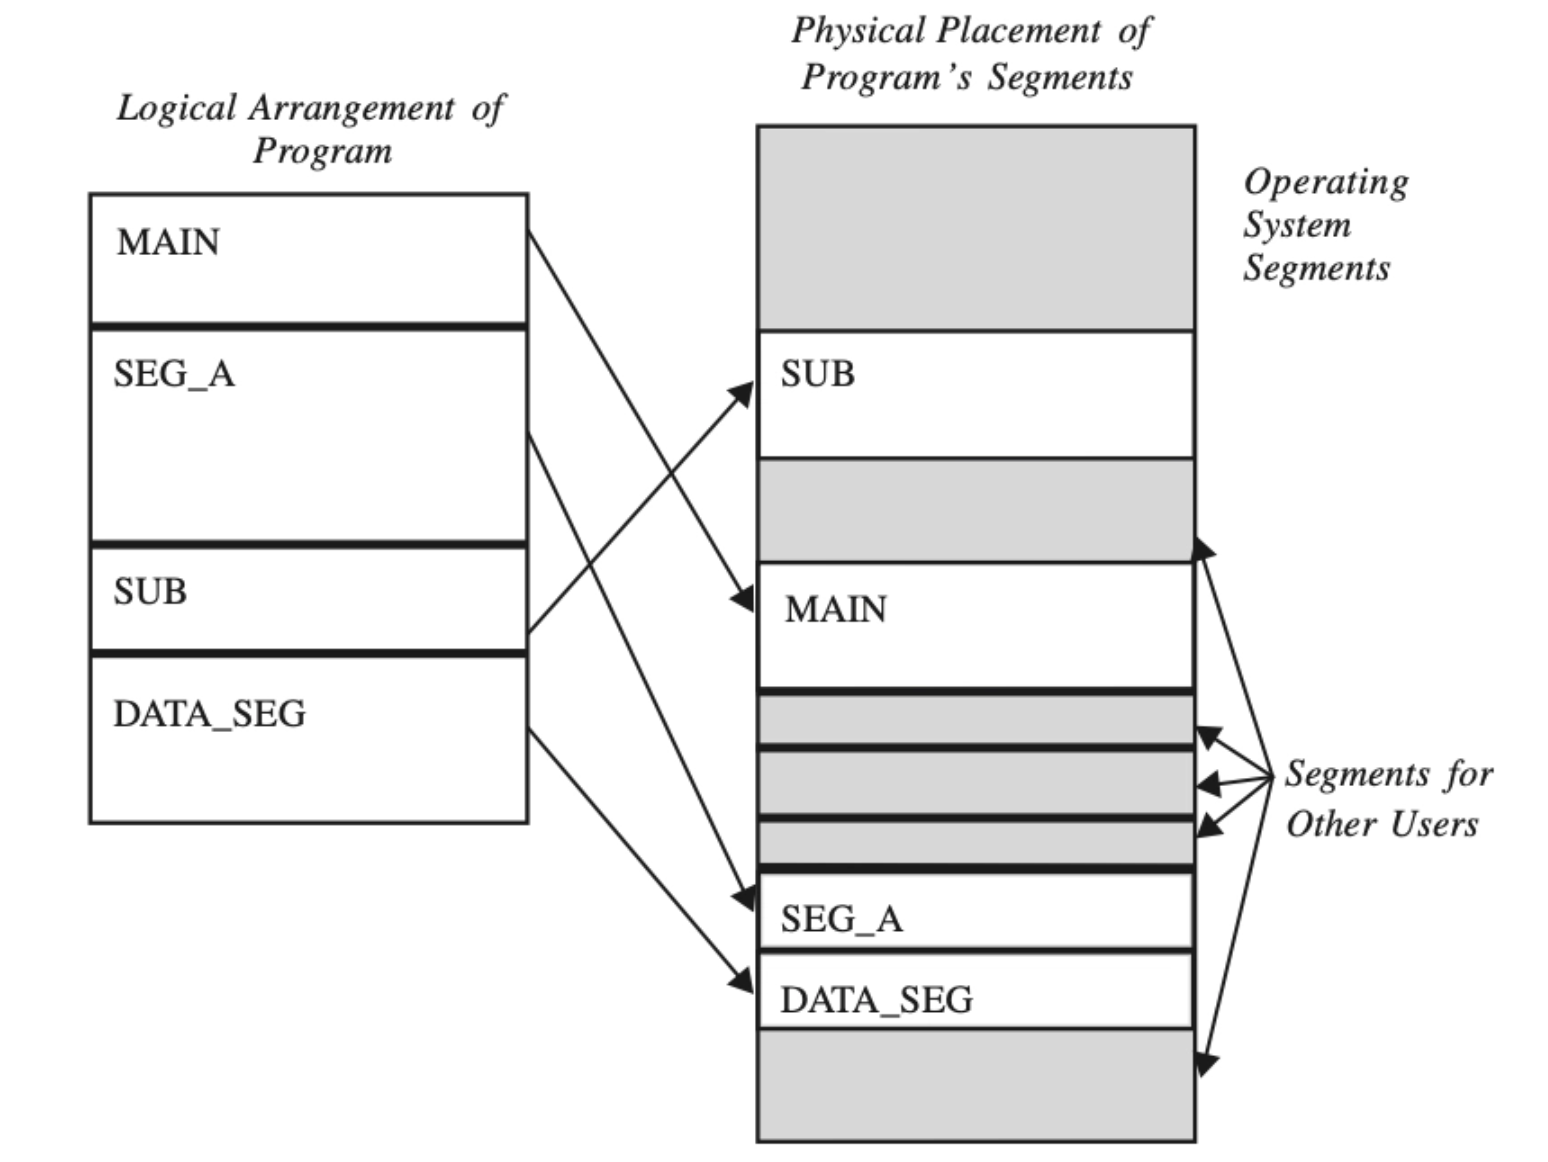
\includegraphics[width=0.8\textwidth]{Screenshot 2026-05-04 alle 13.13.46.png}
\end{center}

La \textbf{Paginazione} risolve il problema delle dimensioni variabili dividendo il programma in pezzi di dimensioni identiche chiamati \textit{pagine}, e la memoria fisica in unità uguali chiamate \textit{page frames}. Utilizza una tabella di traduzione delle pagine, offrendo i vantaggi di sicurezza della segmentazione ma con una gestione della memoria molto più efficiente. Nei sistemi moderni si utilizza spesso la \textbf{Segmentazione Paginata} (Paged Segmentation), un modello ibrido in cui ogni segmento punta a una specifica tabella di paginazione, unendo flessibilità logica ed efficienza fisica.

\begin{center}
    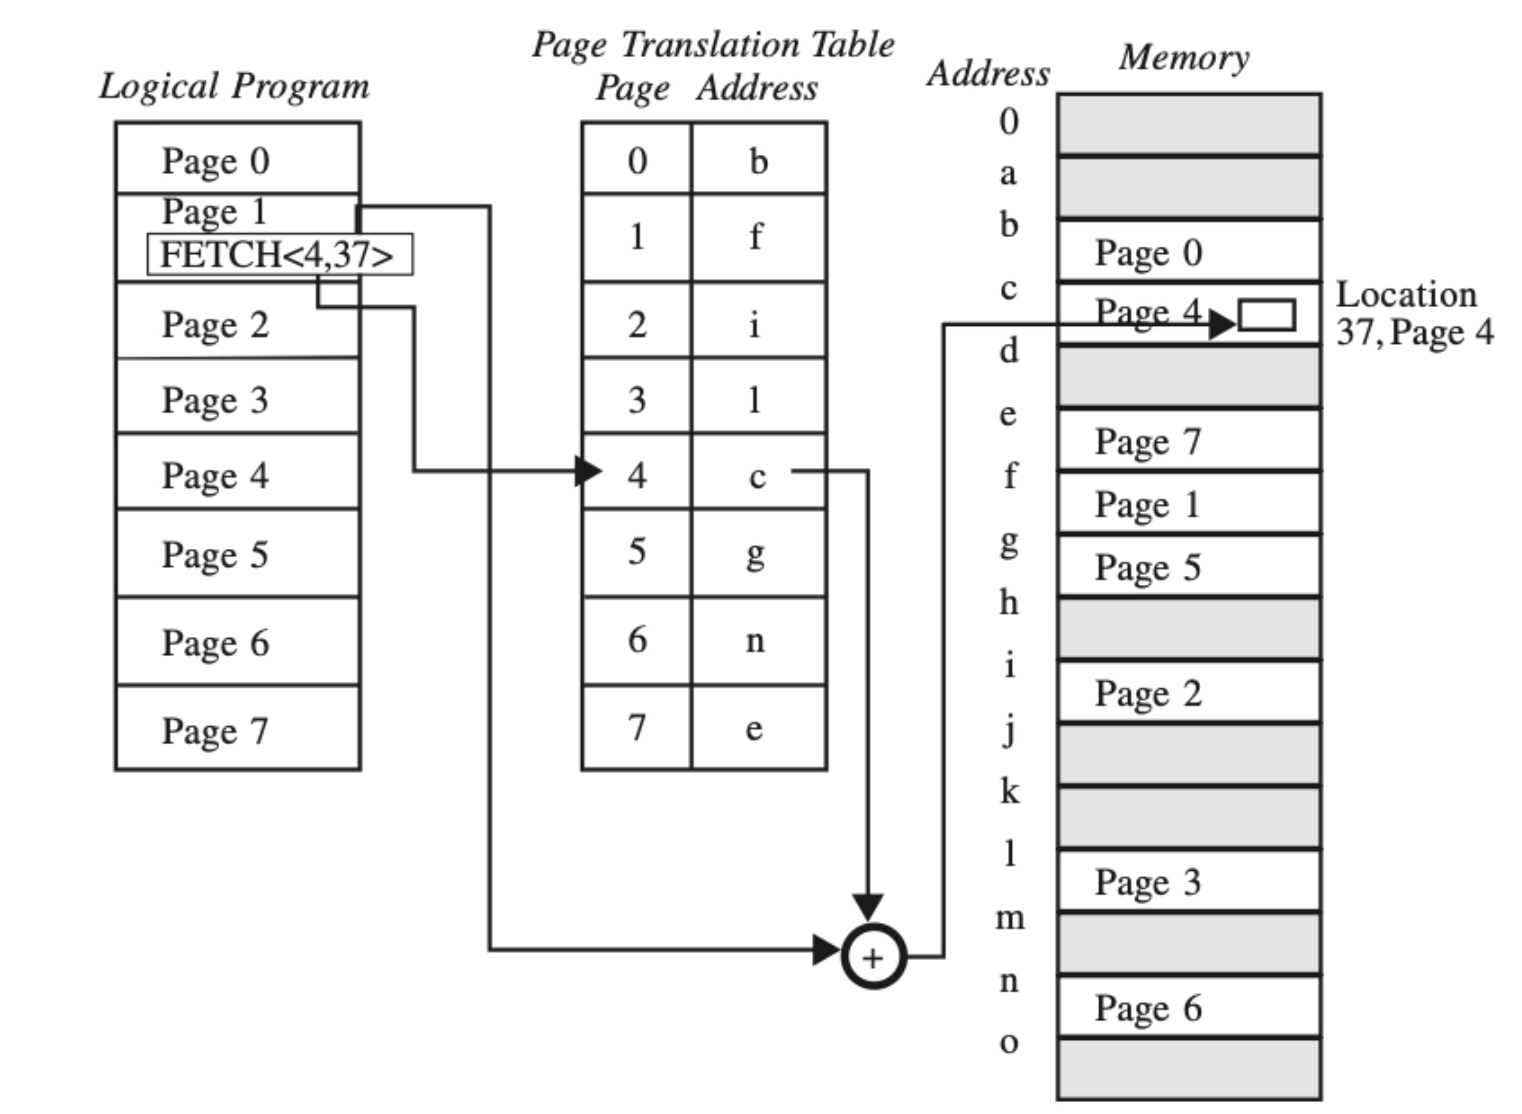
\includegraphics[width=0.8\textwidth]{Screenshot 2026-05-04 alle 13.16.37.png}
\end{center}

\vspace{0.8cm}

\section*{Design Sicuro e Trusted Computing Base (TCB)}

La progettazione di un sistema operativo sicuro si basa su principi architettonici solidi. Tra questi spiccano la semplicità del design, un'architettura a livelli per contenere i danni (encapsulation) e l'adozione di un design kernelizzato. Il nucleo di questa struttura è il \textit{Reference Monitor}, parte del security kernel, che verifica l'esattezza e la completezza dell'applicazione delle policy di controllo degli accessi. Il design deve seguire principi fondamentali come il minimo privilegio, l'economia del meccanismo, l'open design, la mediazione completa e l'accettabilità psicologica (facilità d'uso).

Questi concetti convergono nei \textbf{Trusted Systems}, sistemi operativi che garantiscono la correttezza funzionale (fanno ciò che devono fare), impongono l'integrità dei dati rifiutando comandi non autorizzati e operano con privilegi strettamente limitati. Un sistema fidato possiede una policy di sicurezza ben definita, meccanismi adeguati per farla rispettare e viene sottoposto a valutazioni indipendenti per stabilirne il livello di affidabilità.

Il cuore protettivo del sistema è definito \textbf{Trusted Computing Base (TCB)}. Si tratta dell'insieme di tutto ciò che, all'interno del sistema operativo, è strettamente necessario per far rispettare la policy di sicurezza. Il TCB agisce come un guscio fortificato che protegge tutto ciò che richiede sicurezza nel sistema, basandosi su hardware, processi, file primitivi e memoria protetta. Il TCB monitora costantemente l'attivazione dei processi, il passaggio tra i domini di esecuzione, la protezione della memoria e le operazioni I/O. A livello implementativo, raggruppare tutte le funzioni di sicurezza in un TCB unificato può distruggere la modularità dell'OS e risultare troppo complesso da analizzare. Per questo motivo, si preferisce creare un \textit{security kernel} isolato dalle altre funzioni dell'OS, costruendolo come interfaccia diretta con l'hardware e sviluppando il resto del sistema operativo attorno ad esso.

\end{document}